\section{El lenguaje C++}

\begin{frame}{¿Qué es C++?}
\begin{center}
\begin{tikzpicture}[small mindmap,
    concept color=blue,
    level 1 concept/.append style={font=\tiny,level distance=2.3cm},
    level 2 concept/.append style={font=\tiny,level distance=1.7cm},
    level 3 concept/.append style={font=\tiny},
    every node/.append style={scale=0.9},
    text=white,
    ]
  \node [concept, font=\small] {C++}
    child [grow=25, visible on=<1->] {node[concept] {Es C con ...}}
    child [grow=340, visible on=<2->] {node[concept, visible on=<2->] {Demasiado \ldots}
      child [grow=40, visible on=<3->]{node[concept] {difícil}}
      child [grow=0, visible on=<4->]{node[concept] {bajo nivel}}
      child [grow=320, visible on=<5->]{node[concept] {alto nivel}}
    }
    child [grow=90,visible on=<6->] {node[concept] {Programación}
      child [grow=20,visible on=<7->]{node[concept] {Orientada a objetos}
        child [grow=10]{node[concept] {Clases}}
        child [grow=330]{node[concept] {Jerarquías de clases}}
      }
      child [grow=150,visible on=<8->] {node[concept] {Genérica}
        child [grow=180] {node[concept] {Metapro\-gramción}}
      }
      child [grow=200,visible on=<9->]{node[concept] {Multi\-paradigma}}
    }
    child [grow=180, level distance=2.25cm,visible on=<10->] {node[concept] {Problemas}
      child [grow=200, visible on=<11->] {node[concept] {Buffer overflow}}
      child [grow=150,visible on=<11->] {node[concept] {Goteos de memoria}}
    }
    child [grow=220, visible on=<12->] {node[concept] {Un cajón de sastre}}

  ;
\end{tikzpicture}
\end{center}
\end{frame}

\begin{frame}{¿De donde viene?}
\begin{itemize}
  \item \pause Influencias de alto nivel.
    \begin{itemize}
      \item Lenguajes de abstracción de propósito general.
        \begin{itemize}
          \item Simula.
        \end{itemize}
      \item Lenguajes de abstración de dominio específico.
        \begin{itemize}
          \item FORTRAN, COBOL.
        \end{itemize}
    \end{itemize}
  \item \pause Influencias de bajo nivel.
    \begin{itemize}
      \item Correspondencia directa con el hardware.
        \begin{itemize}
          \item Ensamblador.
        \end{itemize}
      \item Abstracción mínima del hardware.
        \begin{itemize}
          \item BCPL.
          \item C.
        \end{itemize}
    \end{itemize}
  \item \pause Influencias sobre otros lenguajes.
    \begin{itemize}
      \item Java.
      \item C\#.
      \item C (C11).
    \end{itemize}
\end{itemize}
\end{frame}

\begin{frame}{¿Qué es C++11/14/17?}
\begin{itemize}
  \item \pause ISO/IEC 14882:2011, 14882:2014, 14882:2017.
  \item \pause Son la siguientes versiones de C++03.
  \item \pause \emph{``Un lenguaje de programación de abstracciones ligeras''} (B. Stroustroup).
  \item \pause C++11.
    \begin{itemize}
      \item Contiene muchas mejoras sobre C++98/03.
      \item Tiene muchos elementos de compatibilidad.
        \begin{itemize}
          \item La raíz histórica de algunos llega hasta 1972.
        \end{itemize}
      \item Evolucionar un lenguaje con miles de millones de línea de código es
      distinto que diseñar un nuevo lenguaje de programación.
    \end{itemize}
  \item \pause Si alguien dice que tiene un lenguaje de programación perfecto:
    \begin{itemize}
      \item Es na\"{i}ve.
      \item Es un vendedor.
    \end{itemize}
\end{itemize}
\end{frame}


\begin{frame}[t]{El comité ISO C++}
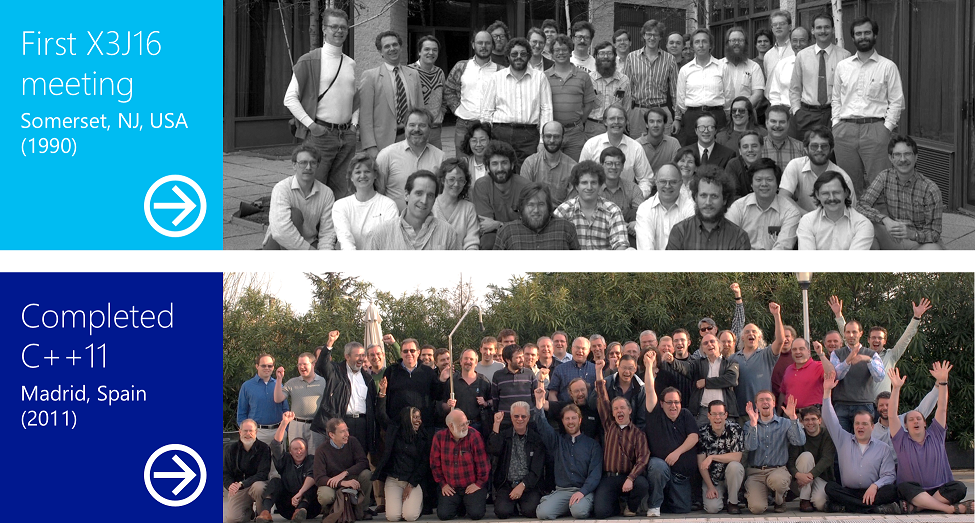
\includegraphics[width=\textwidth]{img/wg21-1990-2011.png}
\end{frame}

\begin{frame}[t]{C++14}
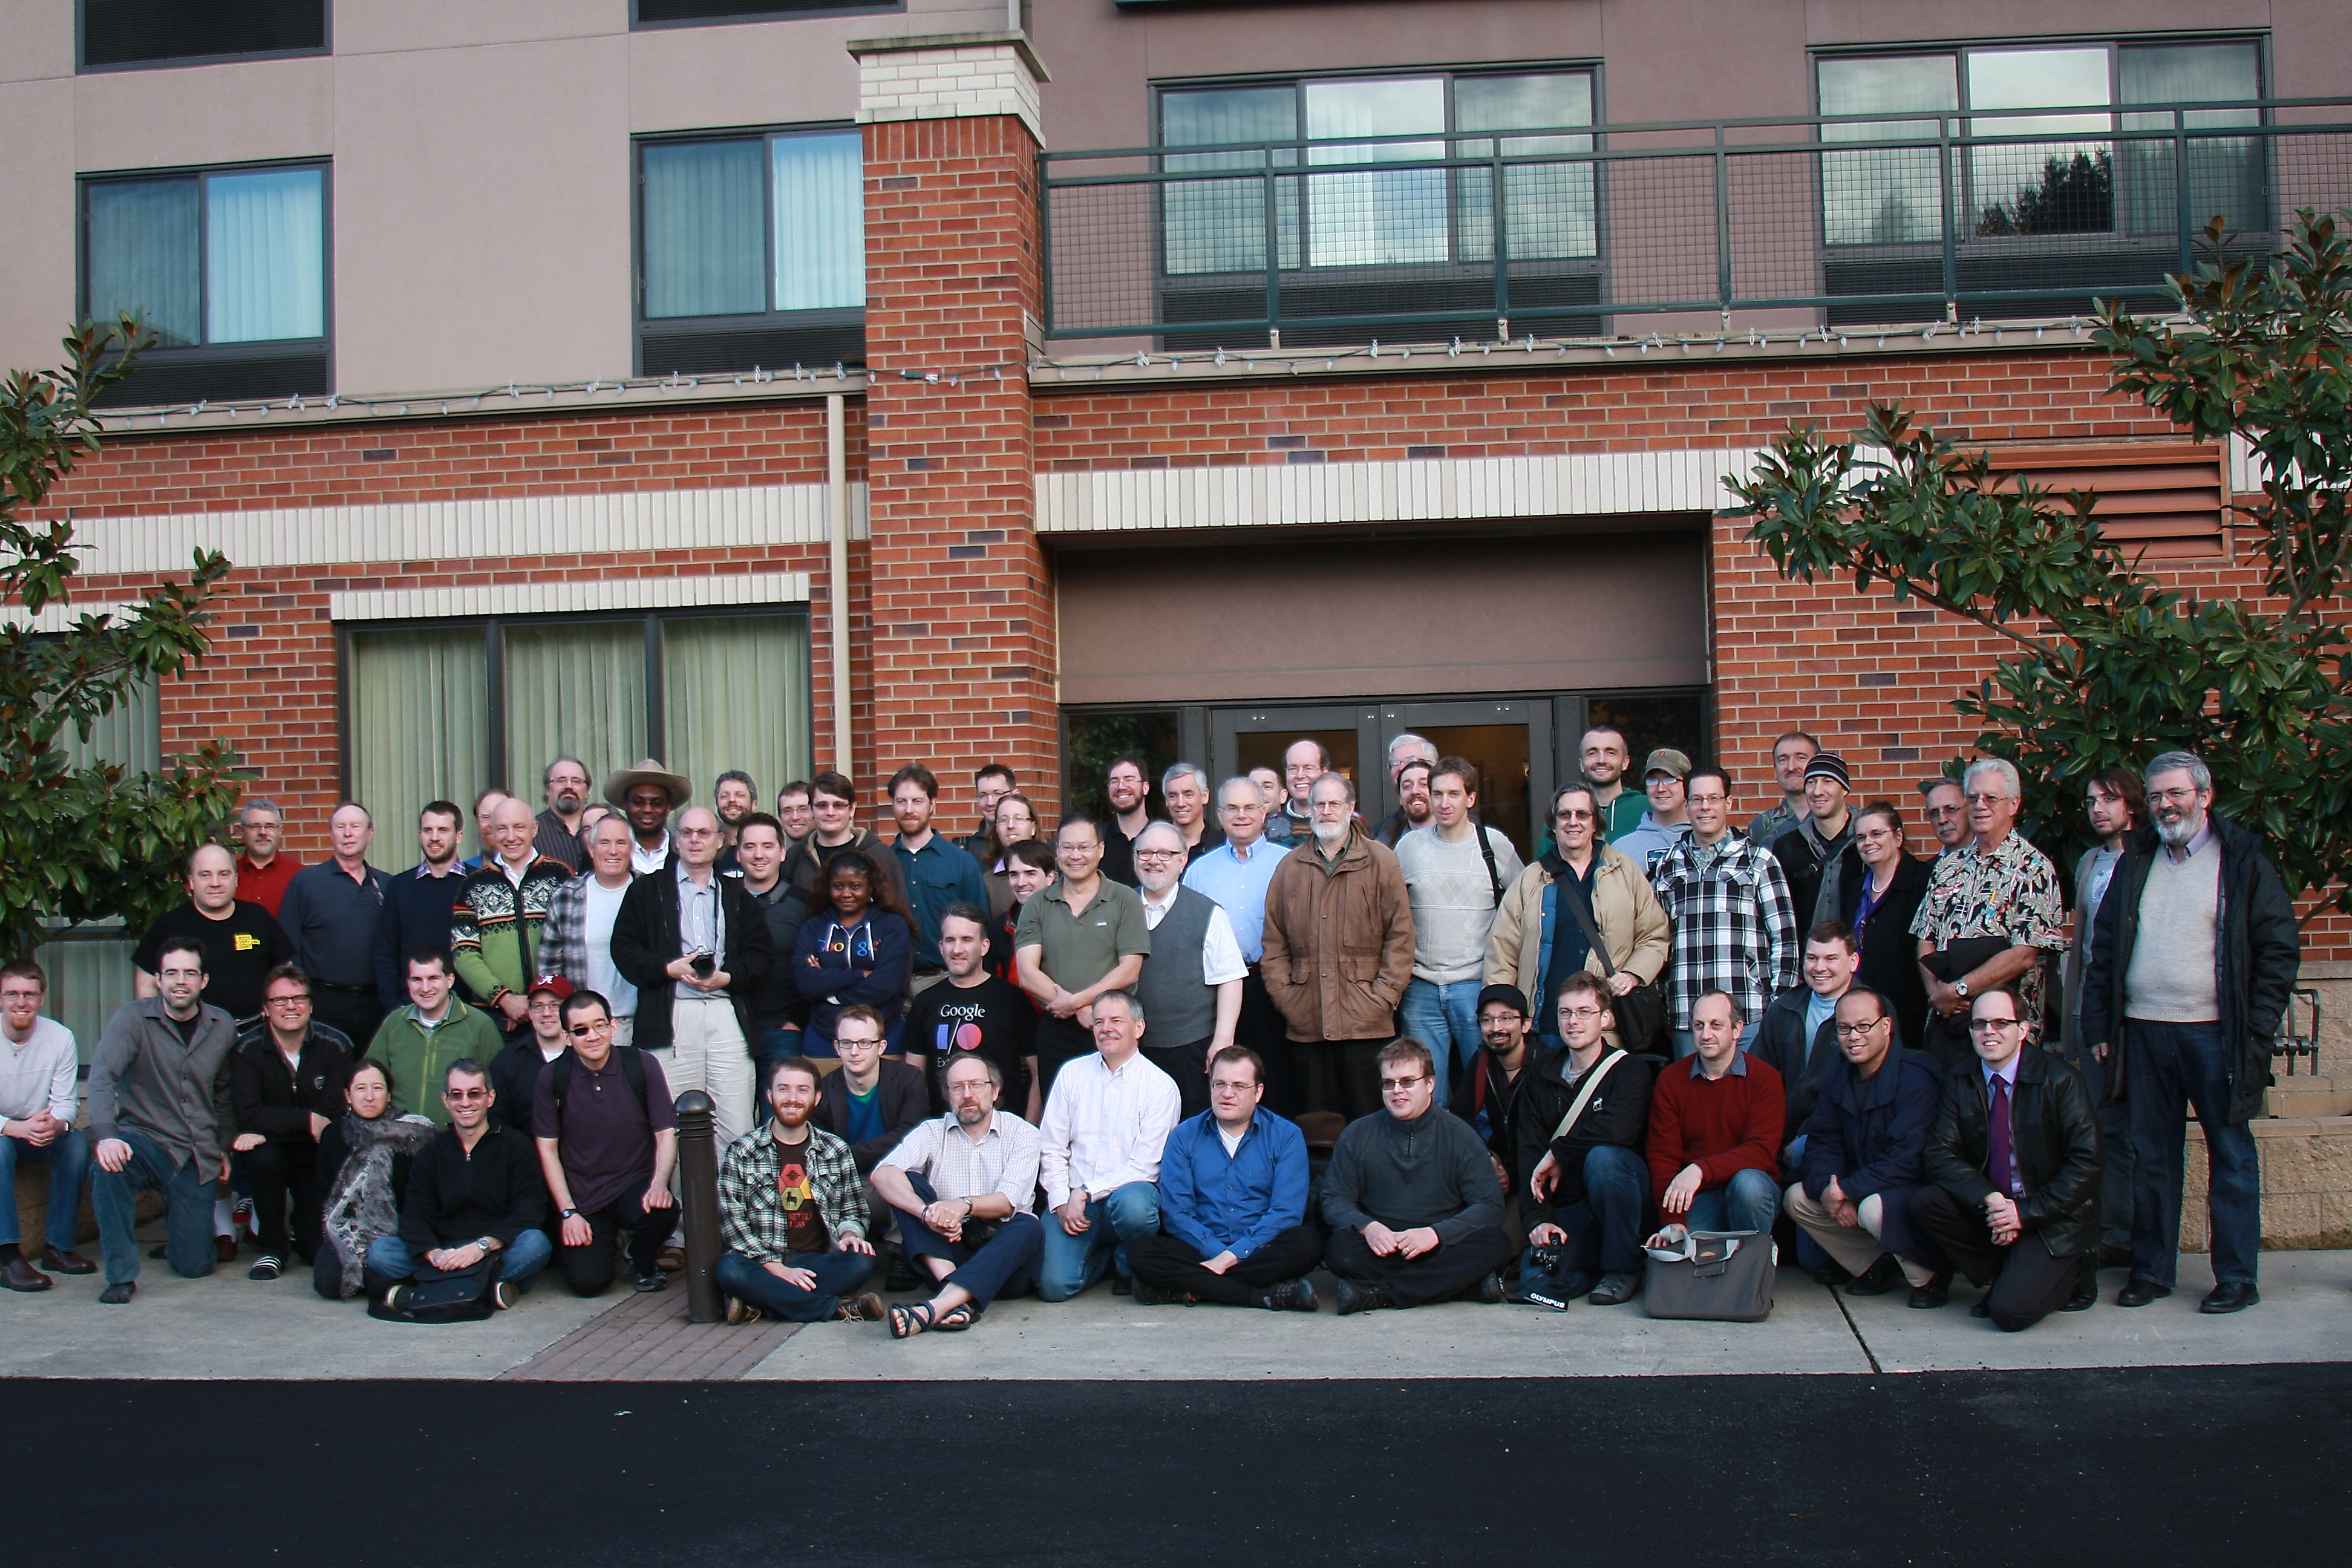
\includegraphics[width=\textwidth]{img/cpp-14.jpg}
\end{frame}

\begin{frame}[t]{C++17}
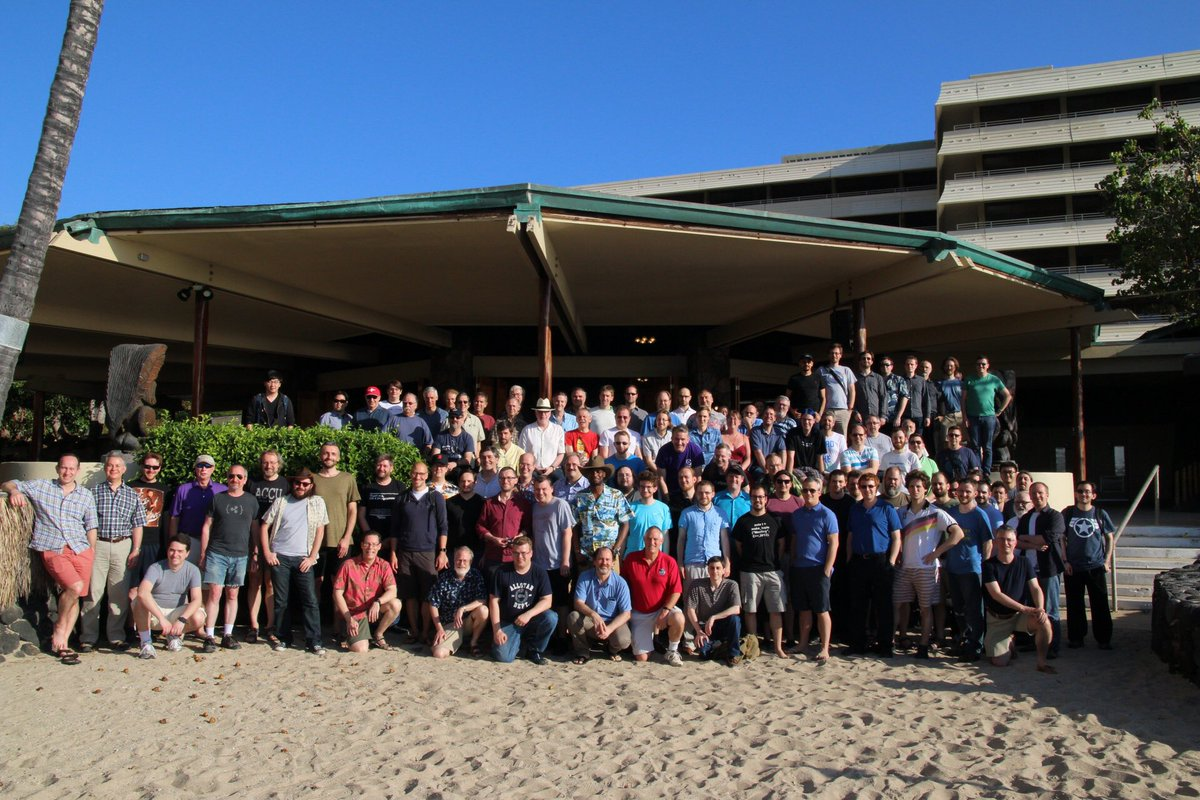
\includegraphics[width=\textwidth]{img/cpp-17.jpg}
\end{frame}

\begin{frame}[t,fragile]{¿Qué pinta tiene?}
	\begin{lstlisting}[escapechar=@]
#include <iostream>
#include <random>
#include <map>

int main() {
  std::mt19937_64 gen;
  std::poisson_distribution dist{2.5}; // mean=2.5
@\pause@
  constexpr int max=10@'@000;@\pause@
  std::map<int,long> freq;@\pause@
  for (int i=0; i<max; ++i) {
    int x = dist(gen);@\pause@
    freq[x]++;
  }
@\pause@
  for (auto [x,f] : freq) {
    std::cout << x << ": " << f << "\n";
  }
}
\end{lstlisting}
\end{frame}

\begin{frame}[t]{Origen}
\begin{columns}[T]
\column{.4\textwidth}
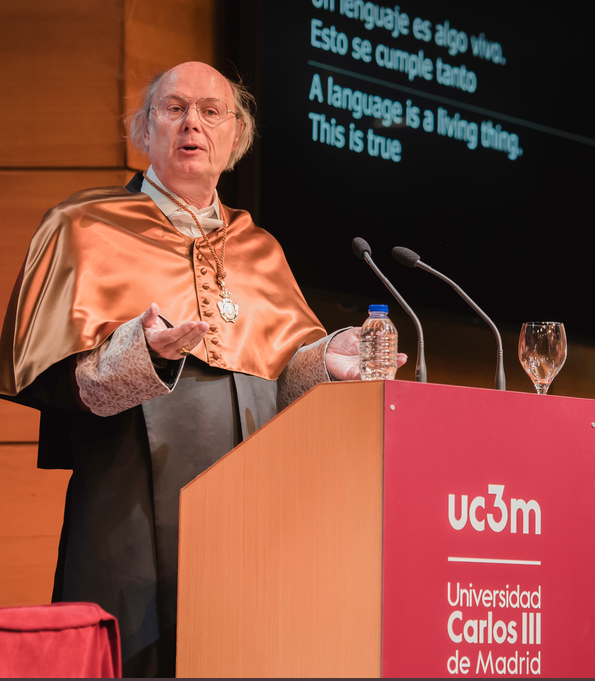
\includegraphics[width=\textwidth]{img/bjarne.png}

\column{.6\textwidth}
\begin{itemize}
  \item Evolución:
    \begin{itemize}
  \item 1979-1982: C with Classes.
  \item 1982-1984: C++ (cfront).
  \item 1986-1989: C++ 2.0 (cfront).
  \item 1988-1990: ARM C++.
  \item 1990: estandarización.
    \end{itemize}
  \vfill
  \item Usuarios:
    \begin{itemize}
      \item 1979: 1
      \item 1980: 16
      \item 1982: 85
      \item 1985: 500
      \item 1987: 4,000
      \item 1989: 50,000
      \item 2019: 4,500,000
    \end{itemize}
\end{itemize}
\end{columns}
\end{frame}

\begin{frame}[t]{Normalización}
\vspace{-1em}
\begin{columns}[T]

\column{.3\textwidth}

\includegraphics[width=\textwidth]{logos/iso.png}

\column{.7\textwidth}
\begin{itemize}
  \item 1998: \textgood{C++98} $\rightarrow$ \textmark{ISO/IEC 14882:1998}.

  \vfill\pause
  \item 2003: \textgood{C++03} $\rightarrow$ \textmark{ISO/IEC 14882:2003}.
    \begin{itemize}
      \item \textemph{Technical Corrigendum}.
    \end{itemize}

  \vfill\pause
  \item 2005: \textgood{C++ TR1} $\rightarrow$ \textmark{ISO/IEC TR 19768}.
    \begin{itemize}
      \item \textemph{C++ Library Extensions}.
    \end{itemize}

  \vfill\pause
  \item 2011: \textgood{C++11} $\rightarrow$ \textmark{ISO/IEC 14882:2011}.

  \vfill\pause
  \item 2014: \textgood{C++14} $\rightarrow$ \textmark{ISO/IEC 14882:2014}. 

  \vfill\pause
  \item 2017: \textgood{C++17} $\rightarrow$ \textmark{ISO/IEC 14882:2017}.

  \vfill\pause
  \item 2020: \textgood{C++20} $\rightarrow$ \textbad{ISO/IEC 14882:????}.
\end{itemize}

\end{columns}
\end{frame}

\begin{frame}{C++ timeline}
\begin{center}
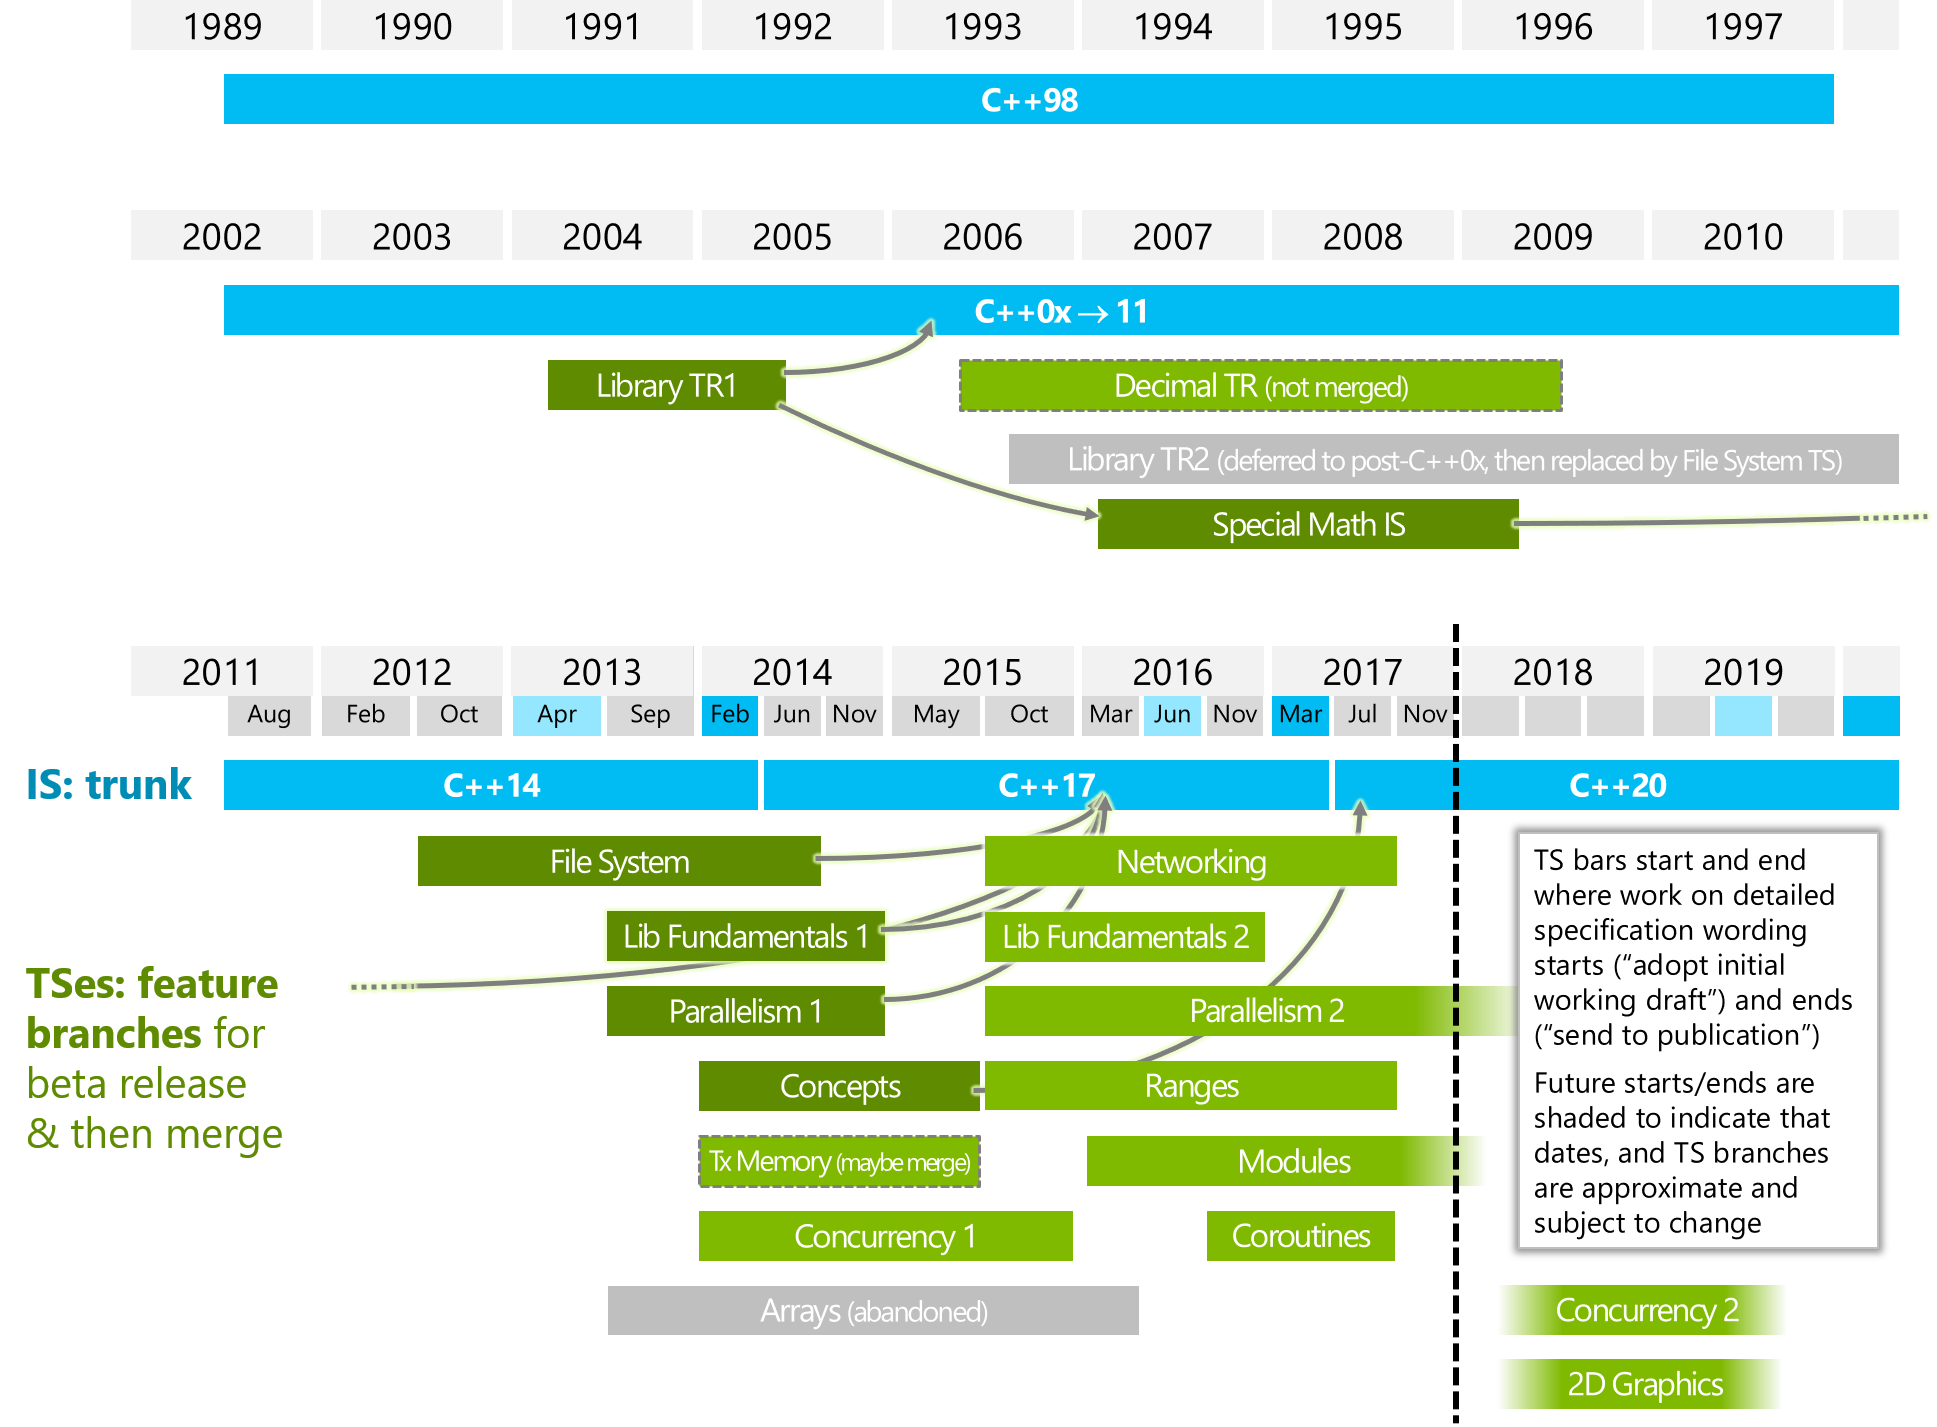
\includegraphics[height=.8\textheight]{img/wg21-timeline.png}
\end{center}
\end{frame}

\begin{frame}[t]{Principios de diseño}
\begin{itemize}
  \item \vfill\pause  Mantener \textmark{compatibilidad} hacia atrás.
  \item \vfill\pause  Mejor \textmark{extender} la biblioteca que el lenguaje.
  \item \vfill\pause  Facilitar el \textmark{diseño} de sistemas y bibliotecas (en vez de dominios concretos).
  \item \vfill\pause  Mejorar la \textmark{seguridad de tipos}.
  \item \vfill\pause  Mejorar el \textmark{rendimiento} y la \textmark{interacción con el hardware}.
  \item \vfill\pause  Principio de \textmark{zero-overhead}.
  \item \vfill\pause  Hacer C++ \textmark{más fácil} de enseñar y aprender.
\end{itemize}
\end{frame}

\begin{frame}{El comité C++}
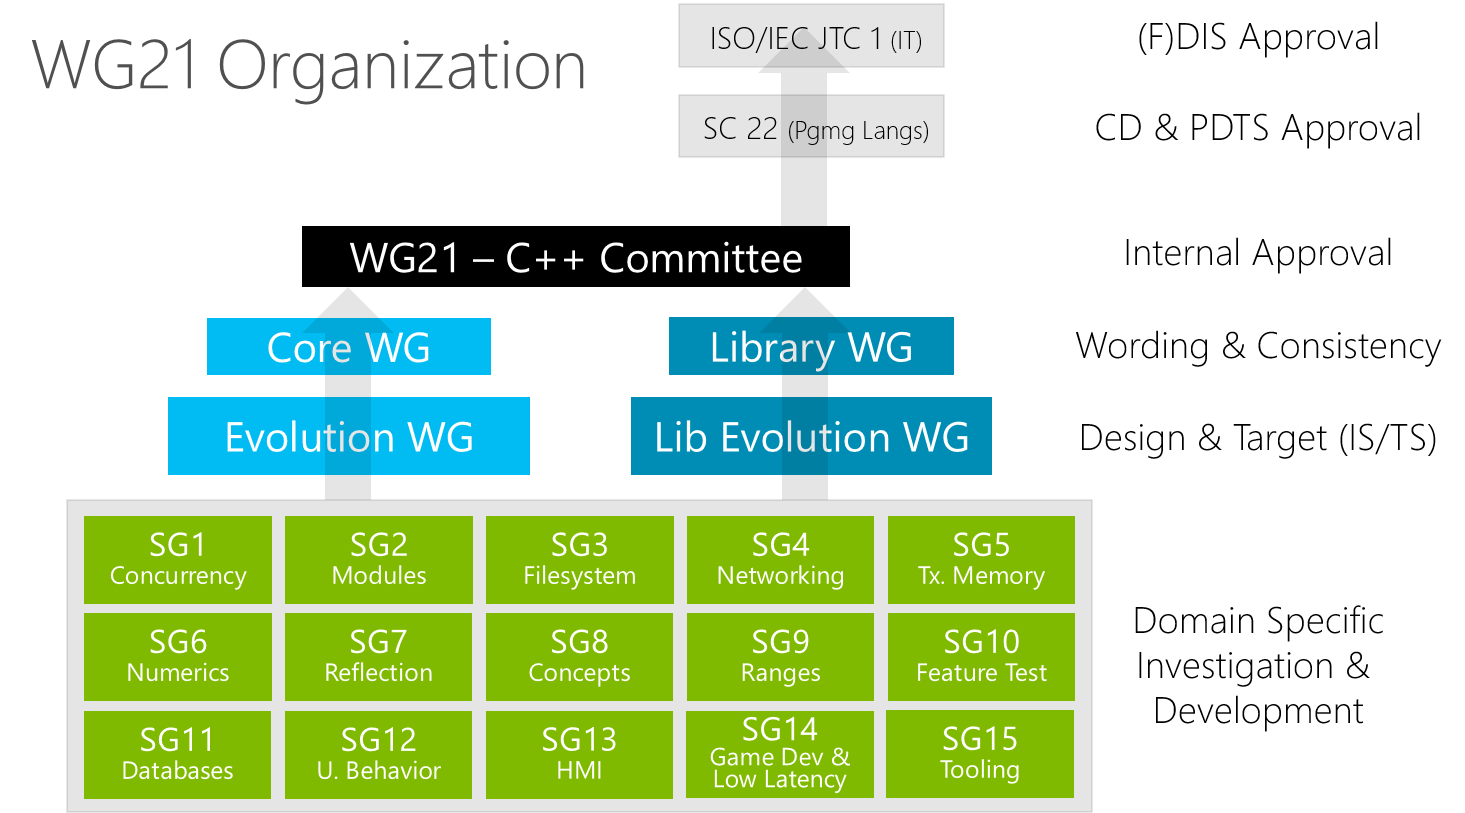
\includegraphics[width=.8\textwidth]{img/wg21-structure.png}
\end{frame}

